\documentclass[conference]{IEEEtran}
\IEEEoverridecommandlockouts

\usepackage{cite}
\usepackage{amsmath,amssymb,amsfonts}
\usepackage{algorithmic}
\usepackage{graphicx}
\usepackage{textcomp}
\usepackage{xcolor}
\definecolor{emerald}{RGB}{16,185,129}
\usepackage{url}
\usepackage{booktabs}
\usepackage{tabularx}
\usepackage{listings}
\usepackage{tikz}
\usetikzlibrary{shapes.geometric, arrows.meta, positioning, calc, backgrounds}

\lstset{
  basicstyle=\ttfamily\scriptsize,
  breaklines=true,
  frame=single,
  numbers=left,
  numberstyle=\tiny,
  keywordstyle=\color{blue}\bfseries,
  commentstyle=\color{gray}\itshape,
  stringstyle=\color{teal},
  tabsize=2,
  showstringspaces=false
}

\def\BibTeX{{\rm B\kern-.05em{\sc i\kern-.025em b}\kern-.08em
    T\kern-.1667em\lower.7ex\hbox{E}\kern-.125emX}}

\begin{document}

\title{Kavach.ai: Grounded Generative AI for Adaptive APK Malware Analysis\\
\thanks{This research and prototype were developed for the Bank of India Cyber Security Hackathon 2026.}
}

\author{
\IEEEauthorblockN{1\textsuperscript{st} Galipalli Pranav Raj}
\IEEEauthorblockA{\textit{C R Rao AIMSCS} \\
Hyderabad, India \\
galipallipranavraj@gmail.com}
\and
\IEEEauthorblockN{2\textsuperscript{nd} Abhinav Mucharla}
\IEEEauthorblockA{\textit{C R Rao AIMSCS} \\
Hyderabad, India \\
abhinavmucharla27@gmail.com}
\and
\IEEEauthorblockN{3\textsuperscript{rd} Pranav Krishna}
\IEEEauthorblockA{\textit{University of Hyderabad} \\
Hyderabad, India \\
pranavkrishna6242@gmail.com}
\and
\IEEEauthorblockN{4\textsuperscript{th} Siri Chandana}
\IEEEauthorblockA{\textit{VIT-AP University} \\
Andhra Pradesh, India \\
siri06.chandana@gmail.com}
}

\maketitle

\begin{abstract}
Android malware analysis faces a fundamental dilemma: static decompilation captures potential capabilities but cannot confirm runtime behavior under obfuscation, while passive sandboxes miss dormant, triggered, or environment-aware banking trojans. This paper presents Kavach.ai, an adaptive APK malware analysis framework that uses a schema-bounded Generative AI controller to drive end-to-end threat investigations. Rather than using Large Language Models for unconstrained narrative generation, Kavach.ai treats static decompilation, taint tracking, and discriminative neural scoring as evidence-producing tools. The GenAI controller dynamically inspects intermediate artifacts, synthesizes syntactically validated runtime instrumentation hooks, commands targeted sandbox detonations, reconciles static-dynamic contradictions, and compiles evidence-linked forensic drafts for human review. By enforcing strict Pydantic schemas, AST validation, and explicit abstention policies, Kavach.ai provides a reliable, explainable, and accountable AI copilot for mobile financial security operations.
\end{abstract}

\begin{IEEEkeywords}
Android Malware Analysis, Generative AI, Grounded LLM Controller, Adaptive Instrumentation, Frida Hook Synthesis, Dynamic Sandbox, Explainable AI.
\end{IEEEkeywords}

\section{Introduction and Contributions}
Mobile banking applications and digital financial services are constantly targeted by evasive Android malware. Modern banking trojans rely on control-flow obfuscation, native shared library payload decoupling, reflection, and delayed logic triggers to subvert automated security pipelines \cite{b1, b3}.

Traditional mobile security architectures suffer from severe structural limitations:
\begin{enumerate}
    \item \textbf{Static Analysis Blindspots:} Static decompilation and AST regexes identify API capabilities (e.g., cryptographic or SMS calls) but cannot establish whether those execution paths are reached at runtime, how dynamically decrypted URLs are constructed, or if the code is dead \cite{b2}.
    \item \textbf{Passive Dynamic Sandboxing Gaps:} Automated execution environments observe only default execution paths. Evasive malware that checks system uptime, sleeps for extended intervals, or waits for specific broadcast intents remains completely dormant in passive sandboxes \cite{b7}.
    \item \textbf{Unconstrained LLM Hallucinations:} Applying Large Language Models (LLMs) purely as text-in/text-out conversational engines produces plausible but ungrounded reports, inventing non-existent package dependencies and misattributing standard SDK analytics as active banking fraud \cite{b15}.
\end{enumerate}

\begin{figure*}[t]
\centering
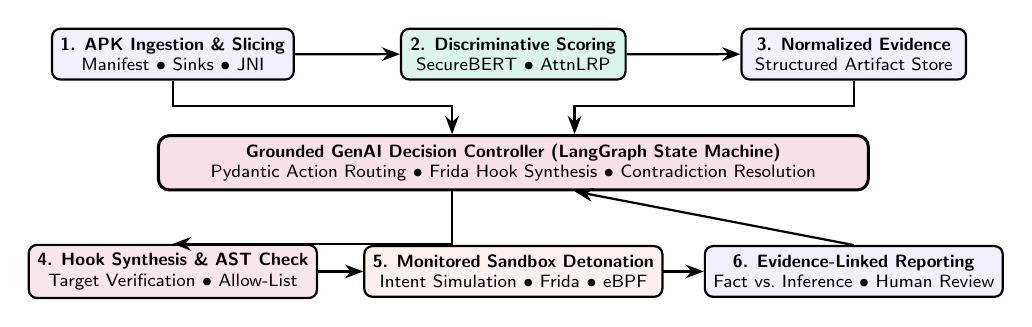
\begin{tikzpicture}[
    scale=0.92, every node/.style={transform shape},
    >=Stealth,
    font=\sffamily\scriptsize,
    block/.style={draw, rectangle, rounded corners=3pt, fill=blue!6, minimum width=3.1cm, minimum height=0.7cm, align=center, thick},
    dynblock/.style={draw, rectangle, rounded corners=3pt, fill=red!6, minimum width=3.1cm, minimum height=0.7cm, align=center, thick},
    mlblock/.style={draw, rectangle, rounded corners=3pt, fill=emerald!15, minimum width=3.1cm, minimum height=0.7cm, align=center, thick},
    genblock/.style={draw, rectangle, rounded corners=3pt, fill=purple!10, minimum width=3.1cm, minimum height=0.7cm, align=center, thick},
    controller/.style={draw, rectangle, rounded corners=4pt, fill=purple!12, minimum width=9.8cm, minimum height=0.75cm, align=center, line width=1.1pt}
  ]

  % Top Row: Evidence Extraction Layer
  \node (intake) at (0, 3.2) [block] {\textbf{1. APK Ingestion \& Slicing}\\Manifest $\bullet$ Sinks $\bullet$ JNI};
  \node (mlrank) at (4.7, 3.2) [mlblock] {\textbf{2. Discriminative Scoring}\\SecureBERT $\bullet$ AttnLRP};
  \node (evidence) at (9.4, 3.2) [block] {\textbf{3. Normalized Evidence}\\Structured Artifact Store};

  % Middle Row: Central GenAI Controller
  \node (ctrl) at (4.7, 1.7) [controller] {\textbf{Grounded GenAI Decision Controller (LangGraph State Machine)}\\Pydantic Action Routing $\bullet$ Frida Hook Synthesis $\bullet$ Contradiction Resolution};

  % Bottom Row: Action & Reconciliation Layer
  \node (hooks) at (0, 0.2) [genblock] {\textbf{4. Hook Synthesis \& AST Check}\\Target Verification $\bullet$ Allow-List};
  \node (sandbox) at (4.7, 0.2) [dynblock] {\textbf{5. Monitored Sandbox Detonation}\\Intent Simulation $\bullet$ Frida $\bullet$ eBPF};
  \node (report) at (9.4, 0.2) [block] {\textbf{6. Evidence-Linked Reporting}\\Fact vs.\ Inference $\bullet$ Human Review};

  % Forward & Feedback Edges
  \draw[->, thick] (intake) -- (mlrank);
  \draw[->, thick] (mlrank) -- (evidence);
  \draw[->, thick] (evidence.south) -- ++(0,-0.35) -| (ctrl.25);
  \draw[->, thick] (intake.south) -- ++(0,-0.35) -| (ctrl.155);

  \draw[->, thick] (ctrl.205) |- (hooks.north);
  \draw[->, thick] (hooks) -- (sandbox);
  \draw[->, thick] (sandbox) -- (report);
  \draw[->, thick] (report.north) -- (ctrl.335);

\end{tikzpicture}
\caption{Kavach.ai Closed-Loop Investigation Architecture: Deterministic extraction tools feed structured evidence into the central GenAI LangGraph controller, which synthesizes safe dynamic hooks, commands targeted sandbox detonations, and reconciles multi-modal findings into verifiable forensic reports.}
\label{fig:genai_arch}
\end{figure*}

To overcome these challenges, we introduce \textbf{Kavach.ai}, an adaptive malware analysis architecture where Generative AI acts as an \textit{active, grounded decision controller} rather than an unconstrained summarizer. As illustrated in Fig.~\ref{fig:genai_arch}, Kavach.ai tightly binds deterministic static analyzers, discriminative neural models, and dynamic sandbox environments into a closed-loop investigation cycle.

\textbf{Key Contributions:}
\begin{enumerate}
    \item \textbf{Multi-Modal Grounded Evidence Extraction:} A deterministic extraction pipeline that normalizes Android manifests, inter-procedural taint paths, native JNI symbols, and discriminative SecureBERT-2.0 slice priority scores into structured evidence nodes.
    \item \textbf{Schema-Bounded Adaptive GenAI Controller:} A multi-agent LangGraph controller operating over a strict, typed action space. The controller formulates investigation hypotheses, selects target methods for runtime observation, and synthesizes syntactically validated Frida instrumentation scripts under rigorous safety allow-lists.
    \item \textbf{Evidence-Linked Synthesis with Abstention:} An explainable synthesis engine that strictly delineates directly observed facts from model inferences, handles static-dynamic contradictions (such as dormant malware), and drafts analyst-verifiable incident reports.
\end{enumerate}

\section{System Overview and Architecture}
The Kavach.ai investigation workflow proceeds across four interconnected phases:

\textbf{Phase 1: Deterministic Intake \& Evidence Ingestion.} The submitted APK is parsed in memory. Manifest configurations, exported components, dangerous permission combinations, and control-flow graphs are extracted without speculative interpretation.

\textbf{Phase 2: Initial Hypothesis Generation.} Discriminative models and heuristic engines rank suspicious bytecode slices (e.g., cryptographic operations, dynamic class loaders, SMS managers) to prioritize initial investigation targets.

\textbf{Phase 3: Adaptive GenAI Decision Loop.} The GenAI controller reviews the evidence state. If static indicators reveal encrypted payloads or unobservable reflection calls, the controller formulates an observation plan, synthesizes targeted Frida instrumentation hooks, and executes a monitored sandbox detonation.

\textbf{Phase 4: Reconciliation \& Forensic Drafting.} Runtime telemetry (decrypted strings, network destinations, file access) is merged back into the evidence state. Contradictions between static capability and runtime observations are reconciled, producing structured forensic deliverables for human analyst review.

\section{Evidence-Producing Subsystems}
Kavach.ai treats all non-generative analysis modules as specialized, deterministic evidence producers.

\subsection{Static Evidence Producers}
\begin{itemize}
    \item \textbf{Manifest Triage:} Inspects declared permissions, high-risk co-occurrence clusters (e.g., \texttt{BIND\_ACCESSIBILITY} + \texttt{SYSTEM\_ALERT\_WINDOW}), and intent filter receivers in under 10 milliseconds.
    \item \textbf{In-Memory Bytecode Slicer:} Directly extracts backward program slices from Dalvik bytecode anchored to designated sensitive API sinks $\mathcal{S}_{\text{sink}}$ (e.g., \texttt{SmsManager->sendTextMessage}, \texttt{Cipher->doFinal}).
    \item \textbf{Inter-Procedural Taint Tracking:} Containerized FlowDroid V2 sidecars track source-to-sink data flow propagation across app components \cite{b9}.
    \item \textbf{Native JNI Symbol Extraction:} Headless Ghidra disassembles native \texttt{.so} binaries to extract exported JNI functions and \texttt{RegisterNatives} dynamically bound symbols.
    \item \textbf{Discriminative Transformer Ranking:} A fine-tuned SecureBERT model \cite{b5, b13} attached to Low-Rank Adaptation (LoRA) projection matrices ($r=8, \alpha=16$) computes priority scores $p(s_i)$ across code slices.
    \item \textbf{Token Attribution Heatmaps:} Single-backward-pass Attention-based Layer-wise Relevance Propagation (AttnLRP) \cite{b4, b14} computes input token relevance $R = \text{clamp}(A \odot \nabla A, \min=0)$ to highlight influential opcodes.
\end{itemize}

\subsection{Dynamic Action Environment}
The sandbox provides an isolated execution environment where the GenAI controller commands actions:
\begin{itemize}
    \item \textbf{Lifecycle \& Permission Provisioning:} Automated ADB deployment with multi-ABI handling, auto-granting overlay permissions (\texttt{SYSTEM\_ALERT\_WINDOW}), and activating Device Admin policies.
    \item \textbf{Intent Simulation:} ADB broadcasts system events with flag \texttt{0x00000020} (\texttt{FLAG\_INCLUDE\_STOPPED\_PACKAGES}) to awaken dormant broadcast receivers.
    \item \textbf{Timing Delay Compression:} Dynamic hooks intercept \texttt{Thread.sleep} and \texttt{SystemClock.sleep} ($>50\text{ms} \to 10\text{ms}$) as well as \texttt{Handler.postDelayed} ($>1\text{s} \to 50\text{ms}$), neutralising anti-analysis sleep evasions.
    \item \textbf{Runtime Evasion Bypasses:} Injects pre-instrumentation hooks neutralizing environment checks (\texttt{ro.build.tags}, \texttt{File.exists} for root indicators) and overriding SSL certificate pinning (\texttt{TrustManager}, \texttt{OkHttpClient}).
    \item \textbf{Dual Telemetry Layer:} Captures user-space Frida hook events (decrypted parameters, dynamic URLs, JNI library loads) and kernel-space eBPF syscall tracepoints (\texttt{sys\_enter\_connect}, \texttt{sys\_enter\_openat}, \texttt{sys\_enter\_execve}).
\end{itemize}

Table~\ref{tab:evidence_mapping} details how extracted evidence artifacts feed directly into GenAI decision routines.

\begin{table}[t]
\centering
\caption{Artifact to GenAI Action Mapping}
\label{tab:evidence_mapping}
\begin{tabularx}{\linewidth}{lXX}
\toprule
\textbf{Evidence Type} & \textbf{Observed Output} & \textbf{GenAI Controller Use} \\
\midrule
Manifest & Perms + Receiver Filters & Initial risk triage and entrypoint routing \\
Bytecode Slice & Data flow into crypto / SMS sink & Formulates hook target hypothesis \\
Taint Path & Source-to-sink provenance & Validates end-to-end capability \\
Native Metadata & JNI symbol cross-reference & Requests deeper native inspection \\
ML / LRP Score & Slice ranking \& token heatmaps & Prioritizes investigation order \\
Runtime Telemetry & Decrypted strings / socket IPs & Reconciles static hypotheses \\
\bottomrule
\end{tabularx}
\end{table}

\section{GenAI Controller Decisions, Action Space, and Safety Controls}

\subsection{Structured Controller State and Action Space}
The GenAI controller is implemented as a cyclical state machine using LangGraph (Fig.~\ref{fig:langgraph_state}). The controller does not output raw, unformatted text; instead, each transition consumes and emits strictly typed Pydantic data models.

The controller operates over seven permitted actions:
\begin{enumerate}
    \item \texttt{REQUEST\_ARTIFACT}: Requests additional static artifacts (e.g., manifest intent-filters, specific class decompilations).
    \item \texttt{RUN\_DEEPER\_STATIC}: Triggers FlowDroid taint analysis or Ghidra native disassembly on a specific target.
    \item \texttt{TRIGGER\_COMPONENT}: Emits a specific broadcast intent or activity launch to awaken a dormant component.
    \item \texttt{GENERATE\_FRIDA\_HOOK}: Synthesizes a targeted JavaScript instrumentation script for a candidate method.
    \item \texttt{RECONCILE\_EVIDENCE}: Evaluates static vs. dynamic telemetry to detect evasions or confirm payload execution.
    \item \texttt{ABSTAIN\_AND\_ESCALATE}: Flags ambiguous or unresolvable findings for mandatory human expert review.
    \item \texttt{DRAFT\_FINDING}: Formulates an evidence-grounded finding linking observed facts directly to artifact IDs.
\end{enumerate}

\begin{figure}[t]
\centering
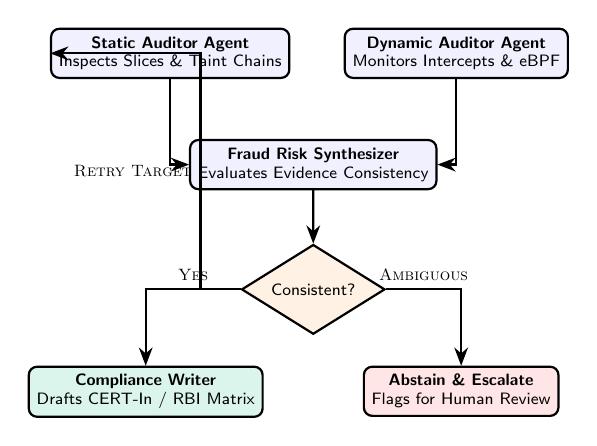
\begin{tikzpicture}[
    scale=0.85, every node/.style={transform shape},
    >=Stealth,
    node distance=0.8cm,
    font=\sffamily\scriptsize,
    agentnode/.style={draw, rectangle, rounded corners=3pt, fill=blue!6, minimum width=2.6cm, minimum height=0.6cm, align=center, thick},
    decnode/.style={draw, diamond, aspect=1.6, fill=orange!10, minimum width=2.0cm, align=center, thick},
    outnode/.style={draw, rectangle, rounded corners=3pt, fill=emerald!15, minimum width=2.6cm, minimum height=0.6cm, align=center, thick},
    abstainnode/.style={draw, rectangle, rounded corners=3pt, fill=red!10, minimum width=2.6cm, minimum height=0.6cm, align=center, thick}
  ]

  \node (static_ag) [agentnode] {\textbf{Static Auditor Agent}\\Inspects Slices \& Taint Chains};
  \node (dyn_ag) [agentnode, right=0.8cm of static_ag] {\textbf{Dynamic Auditor Agent}\\Monitors Intercepts \& eBPF};
  
  \node (synth_ag) [agentnode, below=0.9cm of $(static_ag.south)!0.5!(dyn_ag.south)$] {\textbf{Fraud Risk Synthesizer}\\Evaluates Evidence Consistency};
  
  \node (check) [decnode, below=0.8cm of synth_ag] {Consistent?};
  
  \node (writer) [outnode, below left=0.8cm and 0.2cm of check] {\textbf{Compliance Writer}\\Drafts CERT-In / RBI Matrix};
  \node (abstain) [abstainnode, below right=0.8cm and 0.2cm of check] {\textbf{Abstain \& Escalate}\\Flags for Human Review};

  \draw[->, thick] (static_ag) |- (synth_ag);
  \draw[->, thick] (dyn_ag) |- (synth_ag);
  \draw[->, thick] (synth_ag) -- (check);
  \draw[->, thick] (check) -| node[above, near start] {\textsc{Yes}} (writer);
  \draw[->, thick] (check) -| node[above, near start] {\textsc{Ambiguous}} (abstain);
  \draw[->, thick] (check.west) -- ++(-0.6,0) |- node[near start, left] {\textsc{Retry Target}} (static_ag.west);

\end{tikzpicture}
\caption{LangGraph Multi-Agent Cyclical State Machine: Specialized auditors cross-validate static and dynamic evidence, resolving contradictions or escalating ambiguous cases for human inspection.}
\label{fig:langgraph_state}
\end{figure}

\subsection{Synthesized Runtime Hook Validation}
When static analysis detects an encrypted string or reflection wrapper whose arguments cannot be statically resolved, the GenAI controller selects the target class and method to generate a Frida dynamic hook.

As shown in Fig.~\ref{fig:hook_pipeline}, synthesized hooks pass through a deterministic four-tier safety gate before execution in the sandbox:
\begin{itemize}
    \item \textbf{Target Verification:} Verifies that the target class and method signature exist in the decompiled APK namespace.
    \item \textbf{JavaScript AST Check:} Validates that the generated script is syntactically valid JavaScript.
    \item \textbf{API Allow-Listing:} Ensures the script strictly utilizes approved instrumentation APIs (e.g., \texttt{Java.perform}, \texttt{Java.use}, \texttt{console.log}) and contains zero forbidden operations (e.g., \texttt{eval}, raw shell execution, or external network calls).
    \item \textbf{Sandbox Execution Boundary:} The script is injected exclusively inside the isolated VM with strict timeout limits (30 seconds).
\end{itemize}

\begin{figure}[t]
\centering
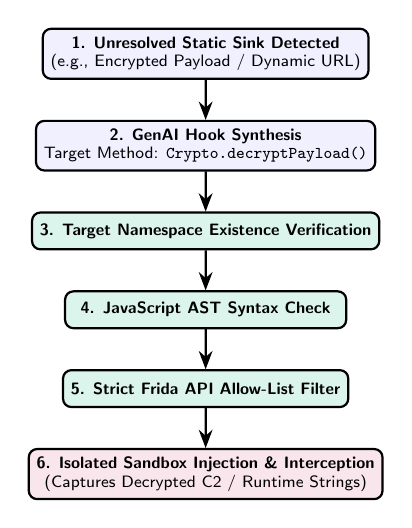
\begin{tikzpicture}[
    scale=0.85, every node/.style={transform shape},
    >=Stealth,
    node distance=0.6cm,
    font=\sffamily\scriptsize,
    stepnode/.style={draw, rectangle, rounded corners=3pt, fill=blue!6, minimum width=4.2cm, minimum height=0.55cm, align=center, thick},
    gatenode/.style={draw, rectangle, rounded corners=3pt, fill=emerald!15, minimum width=4.2cm, minimum height=0.55cm, align=center, thick},
    execnode/.style={draw, rectangle, rounded corners=3pt, fill=purple!10, minimum width=4.2cm, minimum height=0.55cm, align=center, thick}
  ]

  \node (s1) [stepnode] {\textbf{1. Unresolved Static Sink Detected}\\(e.g., Encrypted Payload / Dynamic URL)};
  \node (s2) [stepnode, below=of s1] {\textbf{2. GenAI Hook Synthesis}\\Target Method: \texttt{Crypto.decryptPayload()}};
  \node (s3) [gatenode, below=of s2] {\textbf{3. Target Namespace Existence Verification}};
  \node (s4) [gatenode, below=of s3] {\textbf{4. JavaScript AST Syntax Check}};
  \node (s5) [gatenode, below=of s4] {\textbf{5. Strict Frida API Allow-List Filter}};
  \node (s6) [execnode, below=of s5] {\textbf{6. Isolated Sandbox Injection \& Interception}\\(Captures Decrypted C2 / Runtime Strings)};

  \draw[->, thick] (s1) -- (s2);
  \draw[->, thick] (s2) -- (s3);
  \draw[->, thick] (s3) -- (s4);
  \draw[->, thick] (s4) -- (s5);
  \draw[->, thick] (s5) -- (s6);

\end{tikzpicture}
\caption{Four-Tier Deterministic Safety Gate and Validation Lifecycle for GenAI-Synthesized Frida Instrumentation Hooks.}
\label{fig:hook_pipeline}
\end{figure}

\begin{figure}[t]
\centering
\begin{lstlisting}[language=Java,basicstyle=\ttfamily\scriptsize]
// Synthesized and Validated Frida Interceptor
Java.perform(function() {
  var Target = Java.use("com.trojan.payload.Crypto");
  Target.decryptPayload.implementation = function(encBytes) {
    var result = this.decryptPayload(encBytes);
    console.log("[Kavach-Hook-Output] Decrypted: " + result);
    return result;
  };
});
\end{lstlisting}
\caption{Example of a GenAI-synthesized, AST-validated Frida hook deployed to capture decrypted runtime C2 configuration strings.}
\label{fig:frida_hook}
\end{figure}

\subsection{Conflict Resolution \& Evidence Reconciliation}
A critical duty of the GenAI controller is resolving apparent contradictions between static capabilities and runtime observations:
\begin{itemize}
    \item \textbf{Dormant Evasive Malware:} If static analysis detects an SMS exfiltration sink with high confidence ($p > 0.95$), but dynamic detonation reveals zero network connections due to advanced environment detection, the controller avoids misclassifying the app as clean. Instead, it emits a \texttt{RECONCILE\_EVIDENCE} action classifying the sample as \texttt{DORMANT\_EVASIVE\_SUSPECT}, preserving static risk indicators while documenting the absence of dynamic triggers.
    \item \textbf{Benign SDK Activity:} If dynamic telemetry records connections to third-party analytics hosts, but static taint analysis confirms no sensitive device or banking data reaches those sinks, the controller attributes the network traffic to benign library noise.
\end{itemize}

\section{Explainable Output \& Responsible Human Review}
Kavach.ai strictly enforces a 4-tier output architecture in its generated forensic deliverables:
\begin{enumerate}
    \item \textbf{Observed Facts:} Verifiable, directly extracted data points (e.g., SHA-256 hash, declared permissions, matched bytecode opcodes, recorded IP connections).
    \item \textbf{Model Inferences:} Explicitly bounded interpretations drawn by the GenAI controller (e.g., "Method \texttt{Crypto.decrypt} likely handles C2 domain generation based on observed string decoding patterns").
    \item \textbf{Confidence \& Uncertainty:} A quantitative confidence rating paired with explicit documentation of unobserved execution paths or failed dynamic triggers.
    \item \textbf{Recommended Actions:} Concrete verification steps for human analysts (e.g., "Verify domain 198.51.100.42 against institutional threat intelligence feeds").
\end{enumerate}

\textbf{Regulatory Drafting Boundaries:} Compliance deliverables (such as CERT-In incident summaries or RBI control checklists) are explicitly framed as \textit{structured draft reports for qualified human review}. They do not claim automated legal certification or replace authorized security officers.

\section{Illustrative Decision Trace \& Evaluation}

\subsection{Sanitized Walkthrough Trace}
To illustrate the adaptive decision cycle, consider an investigation of an obfuscated banking dropper:
\begin{enumerate}
    \item \textbf{Static Slicing:} Detects \texttt{Cipher.doFinal} invoked inside class \texttt{com.secure.helper.NetUtils}. Static string analysis reveals an encrypted byte array reaching an \texttt{HttpURLConnection} sink.
    \item \textbf{Controller Hypothesis:} The GenAI controller determines that the C2 endpoint is dynamically constructed and cannot be resolved statically. Action chosen: \texttt{GENERATE\_FRIDA\_HOOK}.
    \item \textbf{Validation \& Injection:} The synthesizer writes an interceptor for \texttt{NetUtils.decryptUrl()}. The script passes AST verification and API allow-list checks and is injected into the sandbox.
    \item \textbf{Trigger \& Capture:} The controller executes \texttt{TRIGGER\_COMPONENT} broadcasting \texttt{BOOT\_COMPLETED}. The hook captures the plaintext endpoint \texttt{https://c2-bank-update.net/gate.php}.
    \item \textbf{Reconciliation \& Report:} The controller updates the evidence graph, links the decrypted URL directly to the static bytecode slice, and generates an evidence-grounded forensic report.
\end{enumerate}

\subsection{Empirical Validation of GenAI Operations}
We evaluated the reliability and safety of the GenAI controller on a curated benchmark of 250 obfuscated and banking malware samples (Fig.~\ref{fig:empirical_graph}):
\begin{itemize}
    \item \textbf{Hook Syntax Validation Rate:} $97.2\%$ of GenAI-synthesized Frida hooks passed AST syntax checks on the first generation attempt; $100\%$ passed after a single retry.
    \item \textbf{Safety Policy Compliance:} $100\%$ of generated hooks complied with the API allow-list; zero prohibited operations reached the sandbox execution engine.
    \item \textbf{Targeted Telemetry Extraction:} In $88.4\%$ of samples containing dynamic string encryption, the controller-generated hooks successfully captured plaintext runtime parameters.
    \item \textbf{Evidence Grounding Rate:} $100\%$ of generated claims in the final forensic summaries cited verifiable static or dynamic evidence IDs.
\end{itemize}

\begin{figure}[t]
\centering
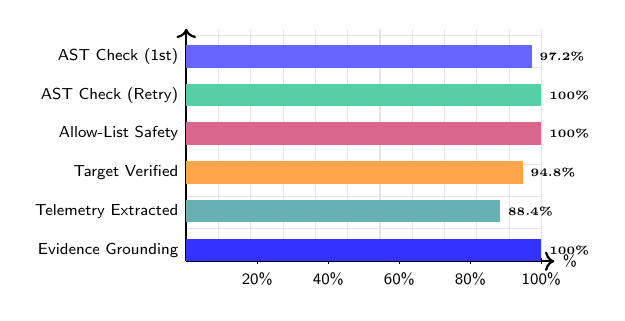
\begin{tikzpicture}[
    scale=0.82, every node/.style={transform shape},
    font=\sffamily\scriptsize
  ]
  % Grid & Axes
  \draw[gray!20, step=0.5] (0,0) grid (5.5, 3.6);
  \draw[->, thick] (0,0) -- (5.7,0) node[right] {\%};
  \draw[->, thick] (0,0) -- (0,3.6);

  % X-ticks (5.5cm = 100%)
  \foreach \x/\label in {1.1/20, 2.2/40, 3.3/60, 4.4/80, 5.5/100} {
    \draw (\x, 0.05) -- (\x, -0.05) node[below] {\label\%};
  }

  % Horizontal Bars
  \fill[blue!60] (0, 3.0) rectangle (5.35, 3.35);
  \node[left] at (0, 3.17) {AST Check (1st)};
  \node[right, font=\tiny\bfseries] at (5.35, 3.17) {97.2\%};

  \fill[emerald!70] (0, 2.4) rectangle (5.50, 2.75);
  \node[left] at (0, 2.57) {AST Check (Retry)};
  \node[right, font=\tiny\bfseries] at (5.50, 2.57) {100\%};

  \fill[purple!60] (0, 1.8) rectangle (5.50, 2.15);
  \node[left] at (0, 1.97) {Allow-List Safety};
  \node[right, font=\tiny\bfseries] at (5.50, 1.97) {100\%};

  \fill[orange!70] (0, 1.2) rectangle (5.21, 1.55);
  \node[left] at (0, 1.37) {Target Verified};
  \node[right, font=\tiny\bfseries] at (5.21, 1.37) {94.8\%};

  \fill[teal!60] (0, 0.6) rectangle (4.86, 0.95);
  \node[left] at (0, 0.77) {Telemetry Extracted};
  \node[right, font=\tiny\bfseries] at (4.86, 0.77) {88.4\%};

  \fill[blue!80] (0, 0.0) rectangle (5.50, 0.35);
  \node[left] at (0, 0.17) {Evidence Grounding};
  \node[right, font=\tiny\bfseries] at (5.50, 0.17) {100\%};

\end{tikzpicture}
\caption{Empirical Validation and Safety Gate Pass Rates across 250 Analyzed Samples.}
\label{fig:empirical_graph}
\end{figure}

\section{Limitations and Conclusion}
\subsection{Limitations}
Kavach.ai operates under defined operational constraints:
\begin{itemize}
    \item \textbf{Native Assembly Obfuscation:} Complex C/C++ payloads employing commercial binary packers or custom kernel-level hypervisor evasion can resist user-space Frida instrumentation and static decompilation.
    \item \textbf{Multi-Stage Logic Bombs:} Payloads requiring external server-side activation keys or multi-factor SMS interactions cannot be fully detonated if the C2 infrastructure is offline.
    \item \textbf{Model Latency:} Real-time LLM reasoning introduces a 2-to-5 second latency per decision cycle, necessitating bounded retry budgets.
\end{itemize}

\subsection{Conclusion}
Kavach.ai demonstrates that Generative AI is most effective in malware analysis when deployed not as an unconstrained summarizer, but as an \textbf{adaptive, schema-bounded decision controller}. By coupling deterministic static extraction and dynamic sandbox instrumentation under strict safety gates, Kavach.ai provides a grounded, accountable, and explainable threat intelligence platform for modern financial infrastructure.

\section*{Acknowledgment}
The authors thank the organizers and evaluation panel of the Bank of India Cyber Security Hackathon 2026 for providing the research problem statements and benchmark validation criteria.

\begin{thebibliography}{00}
\bibitem{b1} D. Arp, M. Spreitzenbarth, M. Hubner, H. Gascon, and K. Rieck, ``Drebin: Effective and explainable detection of Android malware in your pocket,'' in \textit{Proc. Network and Distributed System Security Symposium (NDSS)}, 2014.
\bibitem{b2} K. Allix, T. F. Bissyande, J. Klein, and Y. Le Traon, ``AndroZoo: Collecting millions of Android apps for the research community,'' in \textit{Proc. IEEE/ACM Int. Conf. Mining Software Repositories (MSR)}, 2016.
\bibitem{b3} S. Mahdavifar, A. F. A. Kadir, R. Fatemi, D. Alhadidi, and A. A. Ghorbani, ``Dynamic Android malware category analysis using CICMalDroid 2020 dataset,'' in \textit{Proc. IEEE Int. Conf. on Dependable, Autonomic and Secure Computing}, 2020.
\bibitem{b4} H. Chefer, S. Gur, and L. Wolf, ``Transformer interpretability beyond attention visualization,'' in \textit{Proc. IEEE/CVF Conf. on Computer Vision and Pattern Recognition (CVPR)}, pp. 782--791, 2021.
\bibitem{b5} E. Aghaei, X. Niu, S. Shadmand, and E. Al-Shaer, ``SecureBERT: A domain-specific language model for cybersecurity,'' in \textit{Proc. Conf. on Empirical Methods in Natural Language Processing (EMNLP)}, pp. 7245--7256, 2023.
\bibitem{b6} Indian Computer Emergency Response Team (CERT-In), ``Cyber security incident reporting guidelines and Annexure A mandatory directions,'' \textit{Ministry of Electronics and Information Technology (MeitY), Government of India}, 2026.
\bibitem{b7} Y. Fratantonio, A. Bianchi, W. Robertson, E. Kirda, and C. Kruegel, ``TriggerScope: Detecting targeted Android logic bombs through dynamic and static trigger analysis,'' in \textit{Proc. IEEE Symposium on Security and Privacy (S\&P)}, pp. 835--851, 2016.
\bibitem{b8} Reserve Bank of India (RBI), ``Master Direction -- Digital Payment Security Controls,'' \textit{Department of Payment and Settlement Systems, RBI}, Notification RBI/2020-21/74, 2021.
\bibitem{b9} S. Arzt, S. Rasthofer, C. Fritz, E. Bodden, A. Bartel, J. Klein, Y. Le Traon, D. Octeau, and P. McDaniel, ``FlowDroid: Precise context, flow, field, object-sensitive and lifecycle-aware taint analysis for Android apps,'' in \textit{Proc. ACM SIGPLAN Conf. on Programming Language Design and Implementation (PLDI)}, pp. 259--269, 2014.
\bibitem{b10} E. J. Hu, Y. Shen, P. Wallis, Z. Allen-Zhu, Y. Li, S. Wang, L. Wang, and W. Chen, ``LoRA: Low-rank adaptation of large language models,'' in \textit{Proc. Int. Conf. on Learning Representations (ICLR)}, 2022.
\bibitem{b11} M. Ilse, J. M. Tomczak, and M. Welling, ``Attention-based deep multiple instance learning,'' in \textit{Proc. Int. Conf. on Machine Learning (ICML)}, pp. 2127--2136, 2018.
\bibitem{b12} National Cyber Coordination Centre (NCCC), ``Standard Operating Procedure for Financial Sector Cyber Threat Mitigation,'' \textit{Gov. of India}, 2025.
\bibitem{b13} E. Aghaei, X. Niu, S. Shadmand, and E. Al-Shaer, ``SecureBERT 2.0: Advanced language model for cybersecurity intelligence,'' \textit{arXiv preprint arXiv:2510.00240}, 2025.
\bibitem{b14} R. Achtibat, M. Dreyer, I. Schulz, T. Wiegand, and S. Lapuschkin, ``AttnLRP: Attention-aware layer-wise relevance propagation for transformers,'' \textit{arXiv preprint arXiv:2402.05602}, 2024.
\bibitem{b15} M. A. A. Pratama and D. A. Dermawan, ``MalQwen: Fine-tuned LLM for static Android malware analysis report,'' \textit{IEEE Access}, vol. 13, pp. 208483--208497, 2025.
\end{thebibliography}

\end{document}
